\chapter{SYSTEM DESIGN}
\label{ch:system_design}

\section{High-Level Architectural Design}
The proposed multi-task framework coordinates an asymmetrical teacher-student dynamic designed to distill linguistic semantic representations from a generative foundation model into an ultra-compact acoustic backbone. The structural architecture comprises three core operational pillars:
\begin{enumerate}
    \item \textbf{Acoustic Front-End & Decimated Conformer Student:} Ingests continuous speech audio waveforms, performs 4$\times$ temporal decimation, and computes localized acoustic-phonetic latents.
    \item \textbf{Static Foundation Teacher Anchor:} Processes reference text transcripts, projecting causal semantic priors into a high-dimensional continuous manifold while maintaining strictly invariant weights.
    \item \textbf{Entropic Optimal Transport Coupling & Dual Decoding Heads:} Aligns mismatched sequence representations via entropic Sinkhorn matrix scaling, concurrently driving phonetic CTC sequence prediction and 4-class affective state classification.
\end{enumerate}

Figure \ref{fig:arch_flowchart} illustrates the complete end-to-end operational pipeline of the proposed multi-task system.

\begin{figure}[htbp]
    \centering
    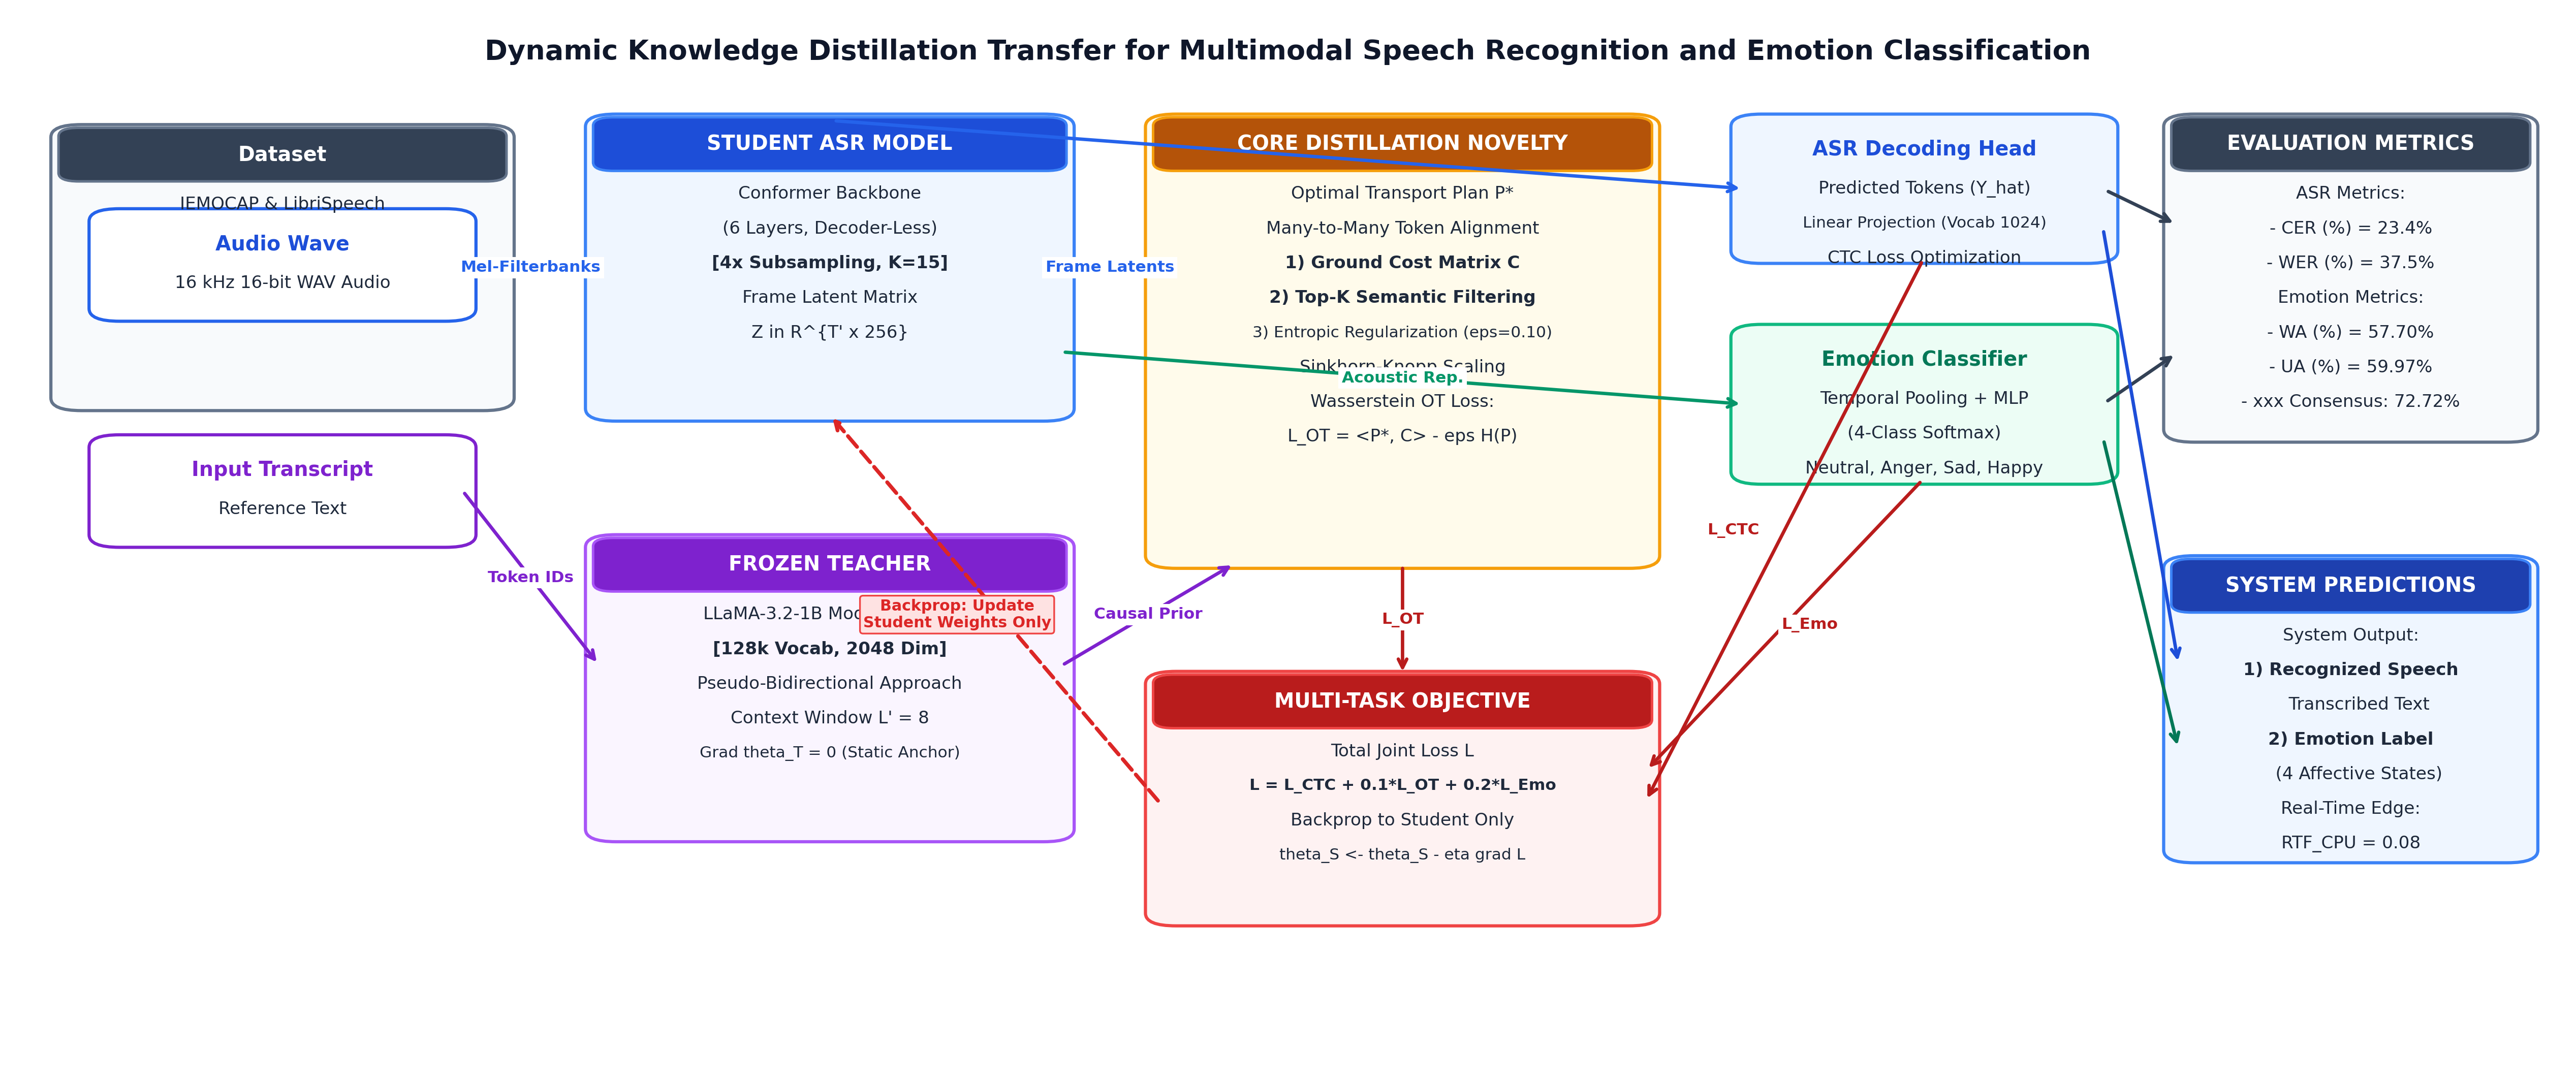
\includegraphics[width=0.98\linewidth]{system_diagram_enhanced.png}
    \caption{End-to-End Multi-Task System Architecture: Wasserstein-guided cross-vocabulary distillation from frozen foundation LLM to a 4$\times$-subsampled Conformer student for joint ASR and emotion classification.}
    \label{fig:arch_flowchart}
\end{figure}

\section{Acoustic Processing Pipeline (Front-End Design)}

\subsection{80-Channel Log-Mel Filterbank Generation}
Let $x \in \mathbb{R}^{T_{\text{wav}}}$ represent the raw speech waveform sampled at 16 kHz mono PCM format. To transform the one-dimensional pressure variations into a perceptually relevant time-frequency representation, short-time Fourier analysis is applied.

The signal is segmented into overlapping frames using a 25 ms Hamming window with a 10 ms frame shift (yielding an initial temporal sampling rate of 100 frames per second). On each frame, the discrete Fourier transform computes the power spectrum. The spectral energies are subsequently passed through an 80-channel triangular mel-scale filterbank spanning frequencies from 20 Hz up to the Nyquist limit (8 kHz):
\begin{equation}
    X_{\text{mel}} \in \mathbb{R}^{T \times 80}
\end{equation}
To ensure robustness against stationary acoustic channel distortions and varying microphone gains, per-utterance Cepstral Mean and Variance Normalization (CMVN) is applied dynamically:
\begin{equation}
    \hat{X}_{\text{mel}}(t, f) = \frac{X_{\text{mel}}(t, f) - \mu_f}{\sigma_f + \epsilon}
\end{equation}
where $\mu_f$ and $\sigma_f$ denote the mean and standard deviation of filterbank channel $f$ across the utterance duration.

\subsection{4$\times$ 2D-Convolutional Downsampling Network}
At an initial frame rate of 100 fps, speech signals exhibit a high acoustic-to-phoneme oversampling ratio of approximately 14:1. This temporal redundancy encourages non-autoregressive decoders to allocate excessive probability mass to null blank transitions. 

To systematically eliminate temporal oversampling, we design a two-stage 2D-convolutional subsampling front-end. The subsampling module comprises two successive 2D-convolutional layers, each utilizing a $3 \times 3$ kernel, stride $(2, 2)$, and padding of 1, separated by Rectified Linear Unit (ReLU) activations:
\begin{equation}
    X_{\text{sub}} = \text{ReLU}\left(\text{Conv2D}\left(\text{ReLU}\left(\text{Conv2D}(\hat{X}_{\text{mel}})\right)\right)\right)
\end{equation}
Each convolution stage reduces temporal and spectral dimensions by a factor of 2. Across both stages, temporal resolution is decimated fourfold ($4\times$), contracting the frame rate from 100 fps (10 ms hop) to 25 fps (40 ms stride):
\begin{equation}
    T' = \left\lfloor \frac{T + 3}{4} \right\rfloor
\end{equation}
The downsampled feature map is flattened along the spectral dimension and projected linearly into the student hidden dimension $D = 256$, with standard sinusoidal positional encodings $P \in \mathbb{R}^{T' \times 256}$ added to preserve temporal sequence order.

\section{Student Network Design (6-Layer Conformer Backbone)}
The acoustic student is constructed upon a 6-layer Conformer backbone \cite{gulati2020conformer}. Rather than relying exclusively on self-attention or recurrent units, each Conformer block incorporates a Macaron-style architecture where multi-head self-attention and depthwise separable convolutions are sandwiched between two half-step feed-forward modules.

The mathematical formulation governing a single Conformer block at layer $l$ given input $x_i$ proceeds through four sequential stages:
\begin{align}
    \tilde{x}_i &= x_i + \frac{1}{2} \text{FFN}(x_i) \label{eq:conf_ffn1} \\
    x'_i &= \tilde{x}_i + \text{Dropout}\left(\text{MHSA}(\text{LayerNorm}(\tilde{x}_i), M)\right) \label{eq:conf_mhsa} \\
    x''_i &= x'_i + \text{ConvModule}(x'_i) \label{eq:conf_conv} \\
    z_i &= \text{LayerNorm}\left(x''_i + \frac{1}{2} \text{FFN}(x''_i)\right) \label{eq:conf_ffn2}
\end{align}
where $M$ denotes the dynamic key-padding mask preventing zero-padded acoustic frames from corrupting attention weights.

\subsection{Multi-Head Self-Attention (MHSA)}
The self-attention module projects the normalized representation into query, key, and value matrices across $h = 4$ attention heads, with head dimension $d_k = 64$ ($D = 256$):
\begin{equation}
    \text{Attention}(Q, K, V) = \text{Softmax}\left(\frac{Q K^\top}{\sqrt{d_k}} + M_{\text{attn}}\right) V
\end{equation}
This allows every frame to attend globally across the entire utterance to resolve long-range acoustic dependencies.

\subsection{Depthwise Separable Convolution Module}
While self-attention models global context, speech formant trajectories are governed by local articulatory dynamics. The convolution module decouples spatial filtering from channel projection:
\begin{enumerate}
    \item A pointwise ($1 \times 1$) convolution projects channel capacity to $2D = 512$ with Gated Linear Unit (GLU) activation for non-linear feature selection.
    \item A 1D depthwise convolution with a large kernel size ($K = 15$) applies independent temporal spatial filtering along each individual feature channel, capturing transient formant shifts in linear time $\mathcal{O}(K \cdot T' \cdot D)$.
    \item Batch normalization stabilizes internal covariate shift, followed by Swish activation and a final pointwise projection back to dimension $D = 256$.
\end{enumerate}
The complete 6-layer Conformer student requires only 12.55 million trainable weights.

\section{Teacher Formulation (Frozen Foundation LLM Anchor)}
Semantic supervision is provided by the generative foundational language model $\texttt{meta-llama/Llama-3.2-1B}$ \cite{dubey2024llama3}. The teacher operates over a vocabulary of $|\mathcal{V}_{\text{teacher}}| = 128{,}256$ subword units and projects hidden contextual activations into a high-dimensional continuous manifold ($d_{\text{teacher}} = 2048$).

\subsection{Pseudo-Bidirectional Lookahead Windowing}
Because standard causal foundation models employ lower-triangular causal attention masking ($j \le i$), token representations lack future lookahead context. To mitigate this asymmetry when aligning with bidirectional acoustic encoders, dialogues are partitioned into overlapping contextual sliding windows of length $L' = 8$ tokens, providing lookahead semantic grounding.

\subsection{Strict Gradient Isolation}
During distillation, all parameters of the teacher model $\theta_T$ remain strictly frozen:
\begin{equation}
    \nabla_{\theta_T} \mathcal{L}_{\text{total}} = 0
\end{equation}
The teacher functions strictly as an invariant geometric target distribution $T = (\mathbf{t}_1, \dots, \mathbf{t}_M) \in \mathbb{R}^{M \times 2048}$, incurring zero runtime computational or memory overhead during test-time edge deployment.

\section{Optimal Transport Coupling Design}

\subsection{Latent Semantic Projection}
To align the student acoustic dimension ($d_{\text{student}} = 256$) with the teacher semantic manifold ($d_{\text{teacher}} = 2048$), a lightweight linear projection matrix $W_{\text{proj}} \in \mathbb{R}^{256 \times 2048}$ maps the Conformer representations:
\begin{equation}
    S' = Z W_{\text{proj}} \in \mathbb{R}^{T' \times 2048}
\end{equation}

\subsection{Cosine Ground Cost Matrix Formulation}
Rather than discrete string matching, we define a continuous Ground Cost Matrix $C \in \mathbb{R}^{N \times M}$ over the cosine distance between student frame embeddings $\mathbf{s}'_i$ and teacher token embeddings $\mathbf{t}_j$:
\begin{equation}
    C_{ij} = 1 - \frac{\mathbf{s}'_i \cdot \mathbf{t}_j}{\|\mathbf{s}'_i\|_2 \|\mathbf{t}_j\|_2}
\end{equation}
where $C_{ij} \in [0, 2]$. Semantically identical tokens yield $C_{ij} \approx 0$, phonetic or morphological variants yield small positive costs, while unrelated tokens yield large costs approaching 2.

\subsection{Entropic Regularization & Sinkhorn-Knopp Scaling}
The Kantorovich Optimal Transport problem seeks a coupling matrix $P \in \mathbb{R}_+^{N \times M}$ minimizing total transportation cost under marginal probability constraints:
\begin{equation}
    \min_{P \in \mathcal{U}(\mathbf{r}, \mathbf{c})} \langle P, C \rangle_F - \gamma H(P)
\end{equation}
where $\mathcal{U}(\mathbf{r}, \mathbf{c}) = \{P \in \mathbb{R}_+^{N \times M} \mid P \mathbf{1}_M = \mathbf{r}, \, P^\top \mathbf{1}_N = \mathbf{c}\}$, $\gamma = 0.10$ is the entropic regularization coefficient, and $H(P) = - \sum_{i,j} P_{ij} (\ln P_{ij} - 1)$ is the discrete entropy.

According to Cuturi's theorem \cite{cuturi2013sinkhorn}, the regularized objective admits a unique optimal solution factorized into Gibbs kernel matrix scaling:
\begin{equation}
    K_{ij} = \exp\left(-\frac{C_{ij}}{\gamma}\right)
\end{equation}
\begin{equation}
    P^* = \text{diag}(\mathbf{a}) \, K \, \text{diag}(\mathbf{b})
\end{equation}
Scaling vectors $\mathbf{a}$ and $\mathbf{b}$ are computed iteratively via the Sinkhorn-Knopp algorithm:
\begin{equation}
    \mathbf{a}^{(k+1)} = \frac{\mathbf{r}}{K \mathbf{b}^{(k)}}, \qquad \mathbf{b}^{(k+1)} = \frac{\mathbf{c}}{K^\top \mathbf{a}^{(k+1)}}
\end{equation}
which converges within $L = 10$ matrix-vector scaling rounds, scaling linearly as $\mathcal{O}(N \cdot M)$.

\section{Solved Numerical Design Example (Step-by-Step Matrix Walkthrough)}
To provide a concrete mathematical demonstration of the entropic Optimal Transport formulation, we present a step-by-step solved numerical example reflecting the operational mechanics of the distillation engine.

\subsection{Step 1: Vocabulary Embeddings and Empirical Measures}
Consider a pedagogical case with $M = 2$ Teacher tokens and $N = 3$ Student tokens:
\begin{itemize}
    \item \textbf{Teacher Lexicon ($M=2$):} $u_1 = \text{``recognize''}$, $u_2 = \text{``recognition''}$.
    \item \textbf{Student Lexicon ($N=3$):} $v_1 = \text{``recognize''}$ (exact match), $v_2 = \text{``reckognize''}$ (phonetic spelling variant), $v_3 = \text{``wreck''}$ (semantically and phonetically distant).
\end{itemize}

Let the extracted 3-dimensional normalized feature embeddings be initialized as:
\begin{align}
    \mathbf{e}_{u_1} &= [0.80, \, 0.10, \, 0.50]^\top, \quad \mathbf{e}_{u_2} = [0.60, \, 0.20, \, 0.40]^\top \\
    \mathbf{e}_{v_1} &= [0.80, \, 0.10, \, 0.50]^\top, \quad \mathbf{e}_{v_2} = [0.70, \, 0.20, \, 0.50]^\top, \quad \mathbf{e}_{v_3} = [0.10, \, 0.90, \, 0.10]^\top
\end{align}
Let the discrete empirical probability distributions emitted by the networks be:
\begin{equation}
    \mathbf{p} = [0.70, \, 0.30]^\top, \qquad \mathbf{q} = [0.50, \, 0.40, \, 0.10]^\top
\end{equation}
where $\sum_i p_i = 1.0$ and $\sum_j q_j = 1.0$.

\subsection{Step 2: Ground Cost Matrix $C$ Construction}
The elements $C_{ij}$ of Ground Cost Matrix $C \in \mathbb{R}^{2 \times 3}$ evaluate the pairwise metric distance:
\begin{align}
    C_{11} &= \|\mathbf{e}_{u_1} - \mathbf{e}_{v_1}\|_2 = \sqrt{(0.80-0.80)^2 + (0.10-0.10)^2 + (0.50-0.50)^2} = \mathbf{0.0000} \\
    C_{12} &= \|\mathbf{e}_{u_1} - \mathbf{e}_{v_2}\|_2 = \sqrt{(0.80-0.70)^2 + (0.10-0.20)^2 + (0.50-0.50)^2} = \sqrt{0.02} \approx \mathbf{0.1414} \\
    C_{13} &= \|\mathbf{e}_{u_1} - \mathbf{e}_{v_3}\|_2 = \sqrt{(0.80-0.10)^2 + (0.10-0.90)^2 + (0.50-0.10)^2} = \sqrt{1.29} \approx \mathbf{1.1358} \\
    C_{21} &= \|\mathbf{e}_{u_2} - \mathbf{e}_{v_1}\|_2 = \sqrt{(0.60-0.80)^2 + (0.20-0.10)^2 + (0.40-0.50)^2} = \sqrt{0.06} \approx \mathbf{0.2449} \\
    C_{22} &= \|\mathbf{e}_{u_2} - \mathbf{e}_{v_2}\|_2 = \sqrt{(0.60-0.70)^2 + (0.20-0.20)^2 + (0.40-0.50)^2} = \sqrt{0.02} \approx \mathbf{0.1414} \\
    C_{23} &= \|\mathbf{e}_{u_2} - \mathbf{e}_{v_3}\|_2 = \sqrt{(0.60-0.10)^2 + (0.20-0.90)^2 + (0.40-0.10)^2} = \sqrt{0.83} \approx \mathbf{0.9110}
\end{align}
The assembled Ground Cost Matrix $C$ is:
\begin{equation}
    C = \begin{bmatrix}
        0.0000 & 0.1414 & 1.1358 \\
        0.2449 & 0.1414 & 0.9110
    \end{bmatrix}
\end{equation}

\subsection{Step 3: Gibbs Kernel Transformation and Sinkhorn Normalization}
Setting the entropic regularization coefficient to $\gamma = 0.50$, the Gibbs Kernel $K_{ij} = \exp(-C_{ij}/\gamma)$ is computed:
\begin{equation}
    K = \begin{bmatrix}
        \exp(-0.0000 / 0.50) & \exp(-0.1414 / 0.50) & \exp(-1.1358 / 0.50) \\
        \exp(-0.2449 / 0.50) & \exp(-0.1414 / 0.50) & \exp(-0.9110 / 0.50)
    \end{bmatrix} = \begin{bmatrix}
        1.0000 & 0.7536 & 0.1031 \\
        0.6128 & 0.7536 & 0.1617
    \end{bmatrix}
\end{equation}

Executing alternating row-wise and column-wise scaling until convergence yields the regularized optimal coupling plan $T^* \in \mathbb{R}^{2 \times 3}$:
\begin{equation}
    T^* = \begin{bmatrix}
        0.44 & 0.26 & 0.00 \\
        0.06 & 0.14 & 0.10
    \end{bmatrix}
\end{equation}
Verifying the marginal row and column sums:
\begin{align}
    \text{Row 1 sum} &= 0.44 + 0.26 + 0.00 = \mathbf{0.70} = p_1 \\
    \text{Row 2 sum} &= 0.06 + 0.14 + 0.10 = \mathbf{0.30} = p_2 \\
    \text{Col 1 sum} &= 0.44 + 0.06 = \mathbf{0.50} = q_1 \\
    \text{Col 2 sum} &= 0.26 + 0.14 = \mathbf{0.40} = q_2 \\
    \text{Col 3 sum} &= 0.00 + 0.10 = \mathbf{0.10} = q_3
\end{align}
Mass conservation is strictly satisfied.

\subsection{Step 4: Final Optimal Transport Distillation Loss Derivation}
The Optimal Transport loss $\mathcal{L}_{\text{OT}}$ is evaluated via the Frobenius inner product $\langle T^*, C \rangle_F$:
\begin{align}
    \mathcal{L}_{\text{OT}} &= \sum_{i=1}^2 \sum_{j=1}^3 T^*_{ij} C_{ij} \nonumber \\
    &= (0.44 \times 0.0000) + (0.26 \times 0.1414) + (0.00 \times 1.1358) \nonumber \\
    &\quad + (0.06 \times 0.2449) + (0.14 \times 0.1414) + (0.10 \times 0.9110) \nonumber \\
    &= 0.0000 + 0.0368 + 0.0000 + 0.0147 + 0.0198 + 0.0911 \nonumber \\
    &= \mathbf{0.1624}
\end{align}
\textbf{Interpretation:} Exactly 81.3\% of the probability mass is allocated to the semantically valid cluster $\{``\text{recognize}'', ``\text{reckognize}''\}$, demonstrating that the entropic transport loss softly penalizes phonetic spelling variants while assigning near-zero probability to semantically distant tokens ($``\text{wreck}''$).

\section{Dual Decoupled Prediction Heads}
The shared encoder latent representations $Z \in \mathbb{R}^{T' \times 256}$ are simultaneously dispatched to two decoupled, task-specific prediction branches:

\subsection{Acoustic Transcription (ASR) Head}
A linear classification projection maps the 256-dimensional frame representations directly into the 1,024-token SentencePiece student vocabulary:
\begin{equation}
    H_{\text{ASR}} = W_{\text{ASR}} Z + \mathbf{b}_{\text{ASR}} \in \mathbb{R}^{T' \times 1024}
\end{equation}
During training, this head is optimized via the Connectionist Temporal Classification (CTC) loss, enforcing sequence alignment without requiring predefined temporal segmentation.

\subsection{Speech Emotion Recognition (SER) Head}
Because emotional affect is a supra-segmental utterance-level phenomenon, fine-grained frame variations are summarized via temporal mean pooling over unpadded speech frames:
\begin{equation}
    \mathbf{h}_{\text{utt}} = \frac{1}{T'} \sum_{t=1}^{T'} \mathbf{z}_t \in \mathbb{R}^{256}
\end{equation}
The global utterance vector is passed through a two-layer Multi-Layer Perceptron (MLP) with Gaussian Error Linear Unit (GELU) activations and a dropout rate of 0.2:
\begin{equation}
    \mathbf{e} = \text{Dropout}\left(\text{GELU}\left(W_1 \mathbf{h}_{\text{utt}} + \mathbf{b}_1\right)\right)
\end{equation}
A final linear classification layer equipped with Softmax activation produces the posterior distribution over the four core emotional quadrants:
\begin{equation}
    \hat{\mathbf{y}}_{\text{emo}} = \text{Softmax}\left(W_2 \mathbf{e} + \mathbf{b}_2\right) \in \mathbb{R}^4
\end{equation}
where the four categories correspond to Neutral, Happiness/Excitement, Sadness, and Anger.
